\section{Methodology and Results}
\label{sec:methodology}

\subsection{Data Description and Pre-Processing}
\label{subsec:data}

The data used for training was obtained from historical options data on the $SPY$ asset from January 2021 to December 2022.
The dataset contains various columns about traded options, indexed by date, including strike prices, future prices, maturities, implied volatilities, among others.
Relevant to our study, the principal columns used were:
\begin{itemize}
    \item \textbf{Underlying}: Price of the underlying asset.
    \item \textbf{Strike}: Option's strike price.
    \item \textbf{Expiration}: Days remaining until the option's expiration.
    \item \textbf{Implied Volatility}: Value for the implied volatility.
    \item \textbf{Date}: Current date, used as the preprocessed set index.
\end{itemize}

Additionally, two columns were calculated to be used as features for the model:
\begin{itemize}
    \item \textbf{Maturity}: Calculated by dividing \textit{Expiration} by 252 (working days in a year) to normalize the maturity time.
    \item \textbf{Risk-free rate}: Risk-free rate obtained from the Federal Reserve Economic Data (FRED) for the corresponding period.
    \item \textbf{Dividend}: Dividend yield paid quarterly by the SPY\@ index.
\end{itemize}

\subsection{Data Preprocessing}
\label{subsec:preprocessing}

The data preprocessing involved several essential steps, predominantly performed to allow the use of the data directly
in the transformer architecture and subsequent use to generate the surface for historical data.
Each of the trained transformers (one for each parameter $\alpha, \rho$, or $\nu$) takes four dimensions as input, which are:
\begin{enumerate}
    \item Time to maturity;
    \item The actual input value for the parameter ($\alpha, \rho$, or $\nu$);
    \item $\mathbf{1}$ if the parameter was calculated for the current day, $\mathbf{0}$ if it was calculated for a fixed set of maturities
    (top 7 most frequent maturities) using the previous day fitted parameters;
    \item Parameter value calculated using the previous day's $\mathbf{P}$, $\mathbf{Q}$ and $\mathbf{R}$ values for same strike and maturity.
\end{enumerate}

The target variable is the scores generated using all candidate points for the current day,
and the model's error function uses the percentage $p = 80\%$ of points and is trained to minimize the quadratic error function of the scores.
For training and testing we also observed that the choice of $\beta = 0.5$ performed best at minimizing the error function.

\subsection{Results and Surface Comparison}
\label{subsec:results}

A baseline linear interpolation implementation for the daily observed points was also used to compare our trained
model's performance by interpolating the points internal to a grid of strikes and maturity dates generated for within the boundary pairs for each day,
that is, no extrapolation was performed due to the hardships of the linear model to predict values outside the observed range.

Our transformer model was trained on the dataset, with about 68 days and 44k observations total.
With an early stopping sensitivity of $\epsilon = 10^{-3}$, the training was performed with a maximum epoch range of $10^{3}$ epochs using the Adam optimizer.
For the implicit layer, we used the Anderson Acceleration algorithm with a maximum of 10 iterations and a convergence threshold of $10^{-6}$.
The training time for the transformer model was approximately 8 minutes and 11 seconds,
while the Monte Carlo preprocessing time was around 21 minutes and 5 seconds for the entire dataset.
Due to the nature of the implicit layer, a simple batch size of 1 was used to avoid memory issues.
The used architecture is a transformer encoder block with 8 attention heads, 2 linear layers with 256 hidden units and 2 implicit layers with 256 and 128 hidden units, respectively.
An illustration of the architecture is shown in \hyperref[fig:figure1]{Figure~\ref*{fig:figure1}}, and a dropout rate of 0.1 was used for the dropout layers.

\begin{figure}[h]
    \begin{center}
        
\includegraphics[width=0.5\textwidth]{images/losses}
        \caption{Historical loss function from on training session data.}
        \label{fig:figure2}
        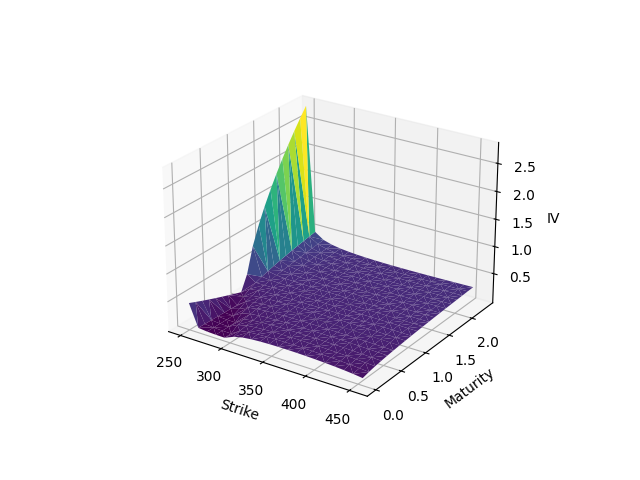
\includegraphics[width=0.5\textwidth]{images/unfitted}
        \caption{Surface generated using a manually optimized SABR model, with all data points, resulting in an out-of-range peak.}
        \label{fig:figure3}
    \end{center}
\end{figure}

\begin{table}[!ht]
    \centering
    \renewcommand{\arraystretch}{1.5} % Adjust the vertical padding
    \resizebox{\columnwidth}{!}{%
        \begin{tabular}{|l|l|l|l|}
            \hline
            Model          & Test Loss (RMSE) & Train time (Transformer) & Preprocess Time (Monte Carlo) \\ \hline
            $SST_{\alpha}$ & 1.21             & $\sim$4m21s              & $\sim$7m50s                   \\ \hline
            $SST_{\rho}$   & 0.72             & $\sim$2m8s               & $\sim$6m34s                   \\ \hline
            $SST_{\nu}$    & 0.75             & $\sim$1m43s              & $\sim$6m41s                   \\ \hline
        \end{tabular}%
    }
    \captionsetup{skip=10pt} % Adjust the caption margin
    \caption{Model training metrics for each of the three SST models.}
    \label{tab:training}
\end{table}

\begin{table}[!ht]
    \centering
    \begin{tabular}{|l|l|l|l|}
        \hline
        Metric                           & Mean time & Standard Deviation \\ \hline
        Execution time on entire dataset & 229.1ms   & 41.2ms             \\ \hline
        Execution time per point         & 2ms       & 1ms                \\ \hline
    \end{tabular}%
    \captionsetup{skip=10pt} % Adjust the caption margin
    \caption{Model performance}
    \label{tab:performance}
\end{table}

For benchmarking the execution time, a small heatup of the model was performed, and the execution time was measured using the Python \texttt{perf\_counter} method.
Separate tests using a linear interpolation with the original points and with the implicit layer were performed to compare the generated surface's error.
The results of the training and testing of the model are shown in \hyperref[tab:training]{Table~\ref*{tab:training}} and \hyperref[fig:figure2]{Figure~\ref*{fig:figure2}}.
The RMSE values for the test data show that the model was able to generalize well to the test data, with the lowest RMSE value for the $\rho$ parameter.
The error values were calculated by comparing the generated surface with the original points, as mentioned in the previous section.


\begin{figure*}
    \label{fig:figure4}
    \begin{center}
        % First row
        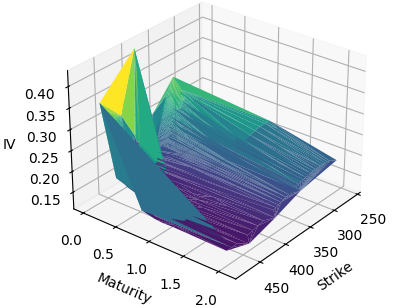
\includegraphics[width=7cm]{images/linear_1}
        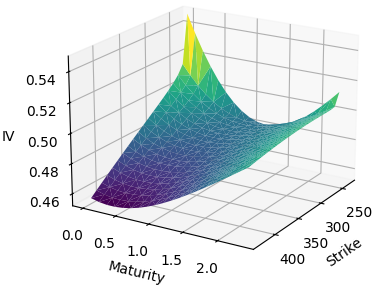
\includegraphics[width=7cm]{images/implicit_1}

        % Second row
        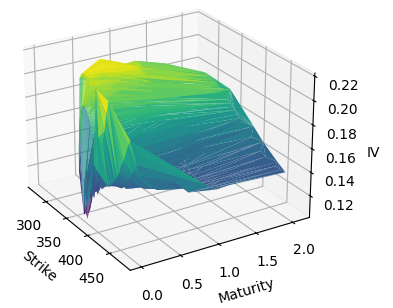
\includegraphics[width=7cm]{images/linear_2}
        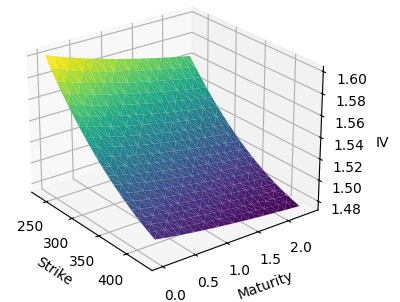
\includegraphics[width=7cm]{images/implicit_2}

        % Third row
        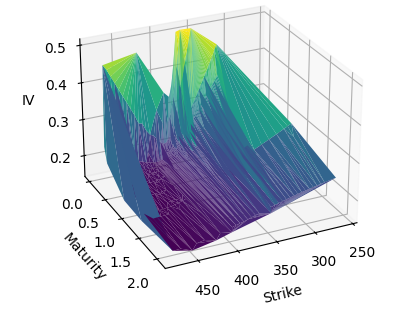
\includegraphics[width=7cm]{images/linear_3}
        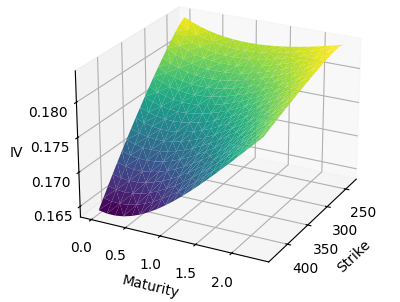
\includegraphics[width=7cm]{images/implicit_3}

        \caption{Surfaces interpolated on test data using a linear interpolation model (left) compared to the SABR model
        fitted with the output of the implicit transformer architecture (right).}
    \end{center}
\end{figure*}
